\documentclass[a4paper, 12pt]{article}

\usepackage{lmodern}
\usepackage{indentfirst}
\usepackage[utf8]{inputenc}
\usepackage{authblk}
\usepackage{fancyhdr}
\usepackage{setspace}
\usepackage{graphicx}
\usepackage{hyperref}
\usepackage{booktabs}
\usepackage{titlesec}
\usepackage[usestackEOL]{stackengine}
\usepackage{float}
\usepackage{adjustbox}
\usepackage[tableposition=top]{caption}
\usepackage{systeme}
\usepackage{amsmath}
\usepackage{mathtools}
\usepackage{commath}

\usepackage[
 left=31.7mm,
 top=25.4mm,
 right=31.7mm,
 bottom=25.4mm
]{geometry}


\usepackage[style=abnt, pretty, usedashes, doi=false, hyperref=false, url=false, language = english]{biblatex}
\addbibresource{master_mutantag.bib} 

\renewbibmacro*{name:andothers}{% Based on name:andothers from biblatex.def
  \ifboolexpr{
    test {\ifnumequal{\value{listcount}}{\value{liststop}}}
    and
    test \ifmorenames
  }
    {\ifnumgreater{\value{liststop}}{1}
       {\finalandcomma}
       {}%
     \andothersdelim\bibstring[\emph]{andothers}}
    {}}

\titleformat{\section}{\centering\large}{}{0em}{\MakeUppercase}[\titlerule]

\renewcommand{\contentsname}{Índice}

\newcommand*\wildcard[2][5cm]{\vspace*{2cm}\parbox{#1}{\hrulefill\par#2}}

\renewcommand\Authfont{\fontsize{14}{14.4}\selectfont}
\renewcommand\Affilfont{\fontsize{10}{10.8}\itshape}

% Title and authors
\title{\vspace{-2.0cm}\textbf{Do we split or we merge? Exploitative interactions increase trait disparity and modularity through coevolution in mutualistic networks}}

\author[1,*]{Lucas Arantes Camacho}
\author[2]{Cecilia Siliansky de Andreazzi}
\author[3]{Lucas Paoliello Medeiros}
\author[4]{Irina Birskis Barros}
\author[5]{Carine Emer}
\author[6]{Carolina Reigada Montoya}
\author[7]{Paulo Roberto Guimarães Junior}
\affil[1]{Programa de pós graduação em Ecologia, Departamento de Ecologia - Instituto de Biociências, Universidade de São Paulo, USP, Rua do Matão, Tv. 14 - Butantã, São Paulo - SP, 05508-090}
\affil[2]{x}
\affil[3]{Department of Civil and Environmental Engineering, MIT, 77 Massachusetts Ave, 02139 Cambridge, MA, USA}
\affil[4]{School of Natural Sciences, University of California, Merced, EUA}
\affil[5]{x}
\affil[6]{x}
\affil[7]{Departamento de Ecologia - Instituto de Biociências, Universidade de São Paulo, USP, Rua do Matão, Tv. 14 - Butantã, São Paulo - SP, 05508-090}
\affil[*]{\textbf{corresponding author: lucas.camacho@usp.br}}
\date{}

% Begin document
\doublespacing
\begin{document}

\setcounter{page}{1}
\begin{center}
\begin{Huge}
Lucas Arantes Camacho

\topskip0pt
\vspace*{\fill}
título tese xxxxxxxxxxxxxxxxxxxxxxxxxxxxxx

title thesis xxxxxxxxxxxxxxxxxxxxxxxxxxxxxx
\end{Huge}
\end{center}

\begin{flushright}
\begin{minipage}{15em}
\begin{singlespace}
Dissertação apresentada ao Instituto de Biociências da Universidade de São Paulo, para a obtenção de Título de Mestre em Ciências, na área de Ecologia.
\bigbreak
Orientador: Prof. Dr. Paulo Roberto Guimarães Junior
\end{singlespace}
\end{minipage}
\vspace*{\fill}
%
\end{flushright}

\begin{center}
\vfill
São Paulo

2020
\end{center}

\newpage

\section*{Ficha catalográfica}

\begin{center}
\vspace{10mm} %5mm vertical space
\fbox{\begin{minipage}{30em}
Camacho, Lucas Arantes
	Título completo da Dissertação
	Número de páginas

	Dissertação (Mestrado) - Instituto de Biociências da Universidade de São Paulo. Departamento de Ecologia.

	1. Coevolução  2. Interações ecológicas  3. Pilhadores 4.Teoria de redes 5. Disparidade de traços  I. Universidade de São Paulo. Instituto de Biociências. Departamento de Ecologia.
\end{minipage}}
\bigbreak
\textbf{Comissão Julgadora:}

\begingroup
  \centering
  \wildcard{Dr(a).	}
  \hspace{1.5cm}
  \wildcard{Dr(a).	}
  \par
\endgroup

\begingroup
  \centering
  \wildcard{Dr(a).	}
  \hspace{1.5cm}
  \wildcard{Orientador}
  \par
\endgroup

\vspace*{\fill}

\end{center}
\newpage

\section*{Dedicatória}
 \thispagestyle{plain}
{\raggedleft\vfill\itshape\Longstack[l]{%
  \textit{Para minha mãe Mirna,}\\
  \textit{e minha vó Nadyr}\\
}\par
}
\newpage

\section*{Epígrafe}
\thispagestyle{plain}
\vfill
 
Um ecossistema se trata de um sistema. Um sistema!
Um sistema mantém certa estabilidade fluída que pode ser destruída por um deslize em apenas um nicho.
Um sistema tem ordem, uma correnteza que flui de um ponto a outro.
Se algo represar a correnteza, a ordem desmoronará.
Os inexperientes talvez só percebam esse desmoronamento quando já for tarde demais.
É por isso que a função mais elevada da ecologia é a compreensão das consequências.

\begin{flushright}
Pardot Kynes, o primeiro planetólogo de Arrakis

(Frank Herbert. \textbf{Duna}. São Paulo: Aleph, 2017)
\end{flushright}
\newpage

\section*{Agradecimentos}
 \thispagestyle{plain}
Agradeço a
\newpage

\tableofcontents
\newpage

\newrefsection
\thispagestyle{plain}
\addcontentsline{toc}{section}{Do we split or we merge? Exploitative interactions increase trait disparity and modularity through coevolution in mutualistic networks}
%\section*{Do we split or we merge? Exploitative interactions increase trait disparity and modularity through coevolution in mutualistic networks}

\begin{singlespace}
\maketitle
\end{singlespace}
\newpage

\addcontentsline{toc}{subsection}{Resumo}
\subsection*{Resumo}
Coevolução, a mudança evolutiva recíproca entre espécies interagentes, é um processo fundamental que influencia a evolução fenotípica de múltiplas espécies. Em comunidades, interações entre indivíduos de espécies diferentes formam redes de interações. Devido a estrutura dessas redes, os efeitos evolutivos podem se propagar diferentemente entre espécies, podendo levar a novas dinâmicas evolutivas. Estas novas dinâmica evolutivas podem ser influenciadas por interações que apresentam consequências distintas para a aptidão dos indivíduos interagentes. Por exemplo, em mutualismos no qual a interação aumenta a aptidão dos indivíduos, emergem redes que podem favorecer  a evolução de modos de vida exploradores de indivíduos mutualistas, reduzindo a aptidão dos indivíduos interagentes. Aqui, exploramos como diferentes frequências de exploração e seus diferentes padrões de interação influenciam a dinâmica coevolutiva em redes mutualísticas. Combinamos  um modelo coevolutivo para redes ecológicas, dados sobre redes empíricas de mutualismos e simulações numéricas para sugerir que a presença de exploração aumenta a disparidade de traços entre espécies. Essa disparidade é caracterizada por grupos de espécies fenotipicamente similares entre si mas distintas de outros grupos de espécies. Porém, considerando espécies exploradoras aquelas que possuem o maior número de interações, a disparidade de traços é variável ou ausente entre diferentes redes de mutualismos. Finalmente, a evolução de traços impulsionada pelas interações de exploração altera a organização das  interações em redes simuladas. Dado que mutualismos podem ser explorados por determinadas formas de vida, nossos resultados mostram como interações de exploração podem mudar a estrutura e a diversidade de traços em redes de mutualismos. \\ 
\textbf{Palavras-chave:} Coevolução, Interações ecológicas, Exploração de mutualismos, Teoria de redes, Disparidade de traços, Pilhadores.

\newpage

\addcontentsline{toc}{subsection}{Abstract}
\subsection*{Abstract}
Coevolution, the reciprocal change mediated by ecological interactions, is a major process affecting the phenotypic evolution of multiple species. In ecological communities, ecological interactions often form networks of interacting species. In this networks, evolutionary changes may cascade across the network, leading to novel evolutive dynamics. This novel dynamics could be drived by interactions with distinct fitness consequences for the individuals. For example, mutualisms, in which interactions increase the fitness of interacting individuals, assemble networks that allow the evolution of exploitative lifestyles, imposing a fitness decrease to the interacting individuals. Here, we explore how exploitation interactions affects the outcome of the coevolutionary dynamics in mutualistic networks. We combined a coevolutive model to ecological networks, empirical mutualistic networks and numerical simulations to suggest that exploitation increases trait disparity between species. Trait disparity is characterized as species groups phenotypically similar between each other but distinct between other species groups. However, considering exploiter species those who maintain the majority of interactions, trait disparity becomes variable between different mutualistic networks. Finally, trait evolution fueled by exploitation interactions change how interactions are organized in the simulated networks. Because exploitation is one possible outcome for mutualisms in natural communities, we showed how exploitation interactions could feedback, reshaping the structure and trait diversity of mutualistic networks. \\
\textbf{Keywords:} Coevolution, Ecological interactions, Mutualism exploitation, Network Theory, Trait disparity, Larceny.
\newpage

\addcontentsline{toc}{subsection}{Introduction}
\subsection*{Introduction}
bla bla

\addcontentsline{toc}{subsection}{Material and Methods}
\subsection*{Material and Methods}

\subsubsection*{The model and the networks}
\cite{abrams_classifying_1987}

\begin{equation} \label{eq:1}
	S_{m} = \sum^{N}_{j} m^{(t)}_{ij}(Z^{(t)}_{j} - Z^{(t)}_{i})
\end{equation}

\begin{equation} \label{eq:2}
  S_{a} = \sum^{N}_{j}v^{(t)}_{ij}(Z^{(t)}_{j} \pm \epsilon_{ij} - Z^{(t)}_{i})
\end{equation}

\begin{equation} \label{eq:3}
  S_{e} = (\theta_{i} - Z^{(t)}_{i})
\end{equation}

\begin{equation} \label{eq:4}
  Z^{(t+1)}_{i} = Z^{(t)}_{i} + \varphi_{i}\{(1 - \gamma_{i})[S_{m} + S_{a}] + \gamma_{i}S_{e}\}
\end{equation}

\begin{equation} \label{eq:5}
  Z^{(t+1)}_{i} = Z^{(t)}_{i} + \varphi_{i}\{(1 - \gamma_{i})[\sum^{N}_{j} m^{(t)}_{ij}(Z^{(t)}_{j} - Z^{(t)}_{i}) + \sum^{N}_{j}v^{(t)}_{ij}(Z^{(t)}_{j} \pm \epsilon_{ij} - Z^{(t)}_{i})] + \gamma_{i}(\theta_{i} - Z^{(t)}_{i})\}
\end{equation}

\begin{equation} \label{eq:6}
  q_{ij} = a_{ij} \frac{e^{-\alpha(Z^{(t)}_{j} - Z^{(t)}_{i})^2}}{\sum_{k, i \neq k} e^{-\alpha(Z^{(t)}_{k} - Z^{(t)}_{i})^2} }
\end{equation}

\begin{equation} \label{eq:7}
MPD = \frac{\sum^{N}_{i}\sum^{N}_{j \neq i} \sqrt{(Z^{(t)}_{j} - Z^{(t)}_{i})^2}}{N(N-1)}  
\end{equation}

\begin{equation} \label{eq:8}
  C_{i} = \frac{k_{i}} {N_{0}}
\end{equation}

\begin{equation} \label{eq:9}
  s_{i} = \frac{C_{i} - \overline{C}}{\sigma}
\end{equation}

\begin{equation} \label{eq:10}
  f(Ch) = \frac{n_{(-+)}}{n_{(-+)} + n_{(++)}}
\end{equation}

\begin{equation} \label{eq:11}
  \systeme*{\abs{Z^{(t)}_{j} - Z^{(t)}_{i}} > b \implies a_{ij} = 0,\abs{Z^{(t)}_{j} - Z^{(t)}_{i}} \leq b \implies a_{ij} = 1}
\end{equation}

\begin{equation} \label{eq:12}
\Delta NODF = NODF_{final} - NODF_{initial}
\end{equation}

\begin{equation} \label{eq:13}
\Delta Q = Q_{final} - Q_{initial}
\end{equation}

\addcontentsline{toc}{subsection}{Results}
\subsection*{Results}
bla

\addcontentsline{toc}{subsection}{Discussion}
\subsection*{Discussion}
bla bla

\addcontentsline{toc}{subsection}{Figures and Tables}
\subsection*{Figures and tables}
\newpage
\begin{singlespace}
\begin{figure}[H]
  \includegraphics[width = \linewidth, height = 19cm]{New_Figura_1.pdf}
  \vspace*{-7mm}
  \caption{...}
  \label{fig:1}
\end{figure}

\begin{figure}[H]
  \includegraphics[width=\linewidth]{New_Figura_2.pdf}
  \vspace*{-7mm}
  \caption{...}
  \label{fig:2}
\end{figure}

\begin{figure}[H]
  \includegraphics[width=\linewidth]{New_Figura_3.pdf}
  \vspace*{-7mm}
  \caption{...}
  \label{fig:3}
\end{figure}

\begin{figure}[H]
  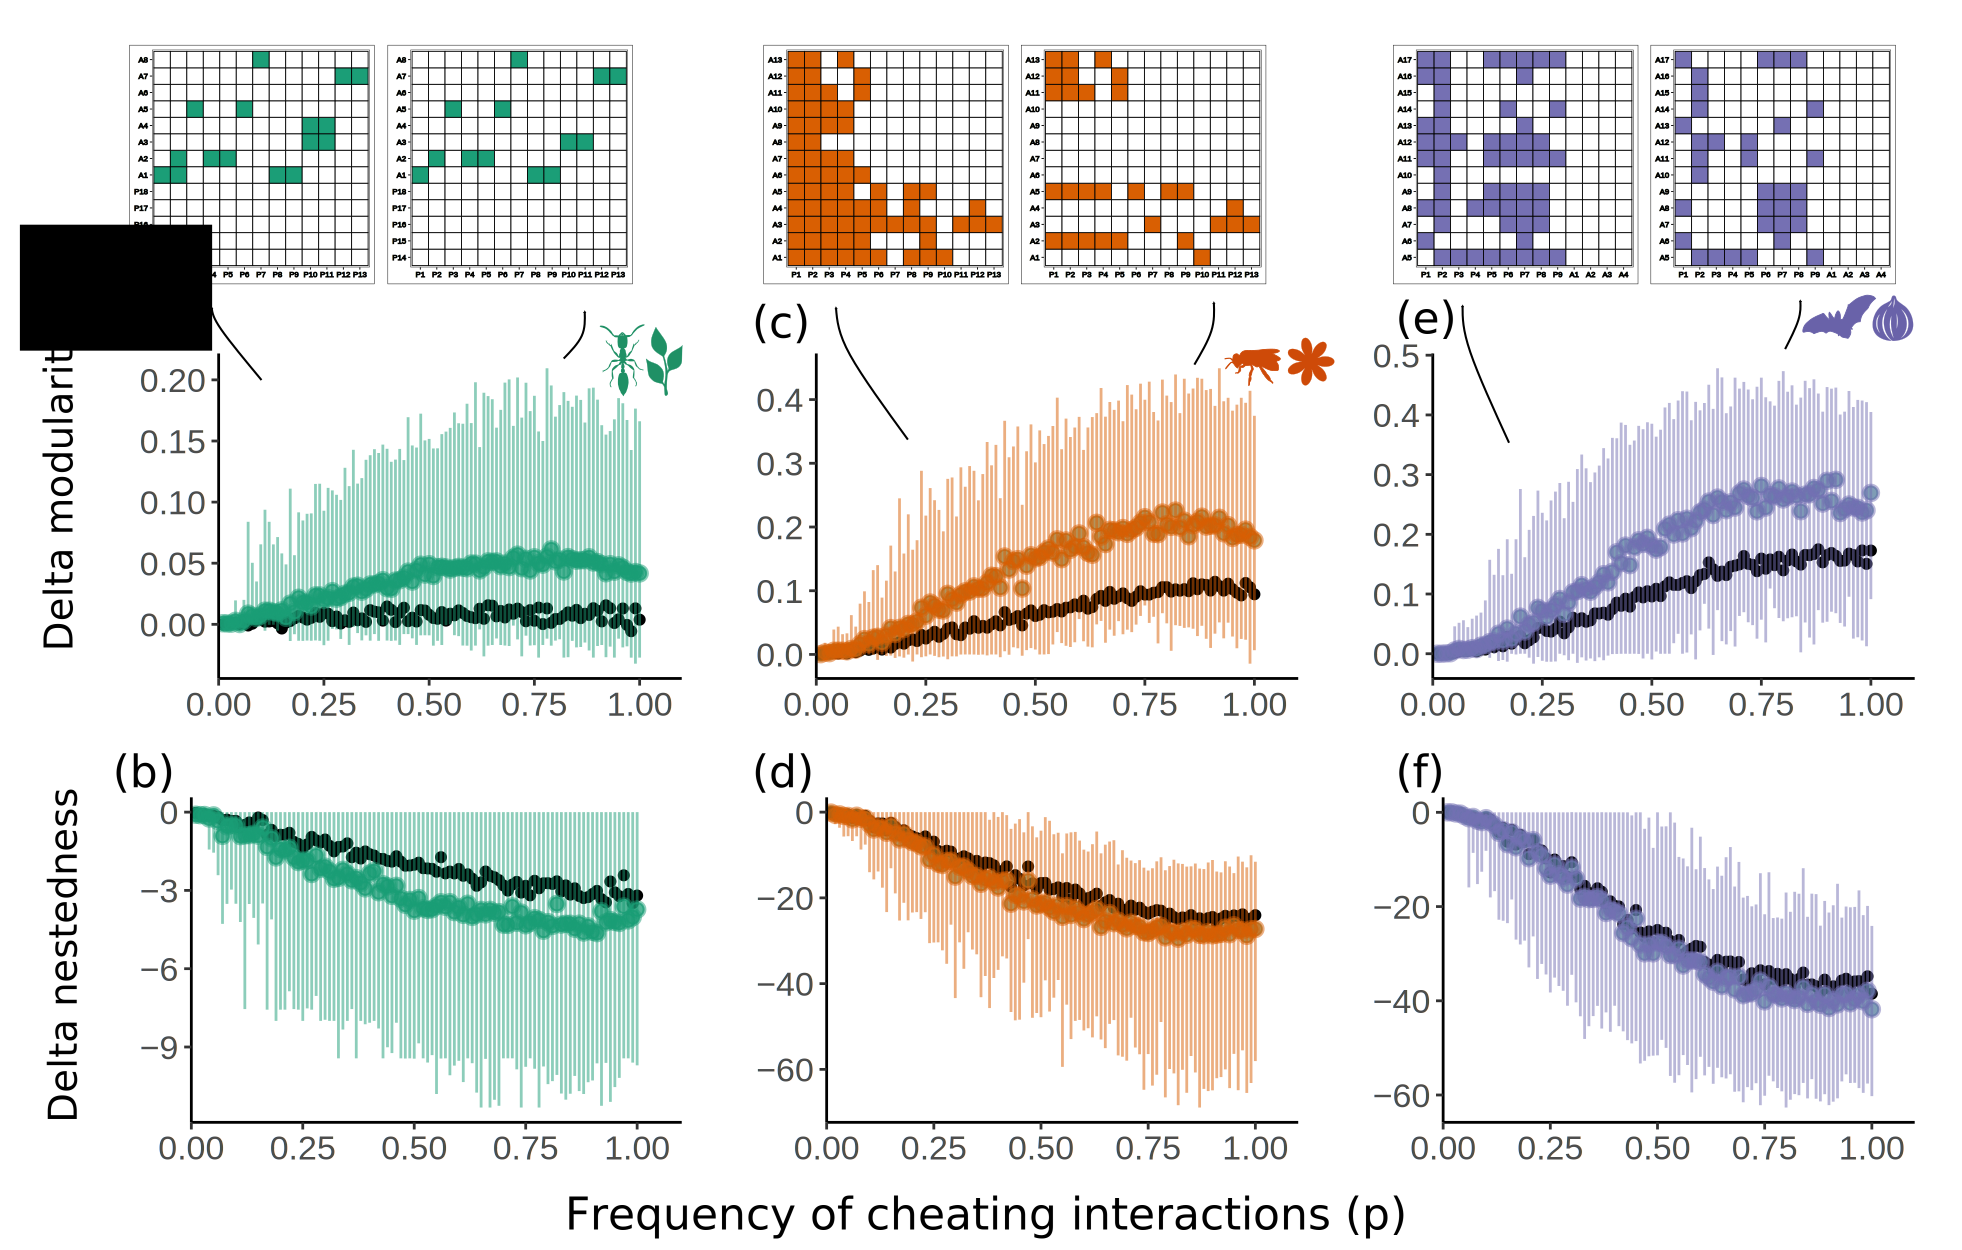
\includegraphics[width=\linewidth]{New_Figura_4.pdf}
  \vspace*{-7mm}
  \caption{....}
  \label{fig:4}
\end{figure}
\end{singlespace}

\begin{table}[H]
\caption{\label{tab:1}Variables and parameters of the model with descriptions and the sample or estimation method.}
\centering
\begin{adjustbox}{width=\columnwidth,center}
\resizebox{\textwidth}{!}{%
\begin{tabular}{ccc}
\hline
\textbf{Parameter} & \textbf{Description}                                                                                                             & \textbf{How it was sampled} \\ \hline
$Z_{i}$            & Initial mean trait value \textit{Z} of species \textit{i}                                                                   & $Z_{i} \sim U(0, 10)$               \\
$\varphi_{i}$              & Parameter composed of the additive genetic variance and phenotypic variance of \textit{Z}                       & Usually fixed as 0.2        \\
$\varepsilon_{ij}$              & Trait barrier to happen the exploitation interaction between species  \textit{i} and \textit{j} & Usually fixed as 5          \\
$\gamma_{i}$             & Strength of abiotic selection for trait change of species \textit{i}                                            & Usually fixed as 0.1        \\
$\theta_{i}$            & $Z_{i}$ optimum value for the environmental selection                                                                            & $\theta_{i} \sim U(0, 10)$                   \\
$\alpha$              & Sensibility of evolutionary effect due to the trait matching between interacting species                                         & Usually fixed as 0.2        \\
\textit{p}         & Probability of an positive effect become negative in a mutualistic network                                                       & $0.01 \leq p \leq 1$                      \\
\textit{b}         & Trait barrier for any interaction happen between species in the network                                                          & Usually fixed as 7          \\ \hline
\end{tabular}}
\end{adjustbox}
\end{table}

\addcontentsline{toc}{subsection}{References}
\subsection*{References}
\begin{singlespace}
\printbibliography[heading = none]
\end{singlespace}
\newpage

\addcontentsline{toc}{section}{Supplemental Informations}
\newrefsection
\renewcommand{\theequation}{S.\arabic{equation}}
\setcounter{equation}{0}
\section*{Supplemental Informations}

\addcontentsline{toc}{subsection}{Coevolution model}
\subsection*{Coevolution model}
\cite{guimaraes_jr_indirect_2017}

\begin{equation}  \label{supeq:1}
  \Delta z^{(t)} = h^{2} \sigma^{2} \frac{\partial{ln \overline{W}}}{\partial z^{(t)}}
\end{equation}

\begin{equation}  \label{supeq:2}
  z_{i, p +} = \sum_{j, j \neq i}^{N} (1 - \gamma_{i})(x^{(t)}_{ij} m^{(t)}_{ij}) + \gamma_{i} \theta_{i}
\end{equation}

\begin{equation} \label{supeq:3}
  z_{i, p -} = \sum_{j, j \neq i}^{N}(1 - \gamma_{i})[(x^{(t)}_{ij} \pm \epsilon_{ij})(v^{(t)}_{ij}\delta_{ij})] + \gamma_{i} \theta_{i}
\end{equation}

\begin{equation} \label{supeq:4}
\abs{x^{(t)}_{ij} \pm \epsilon_{ij} - z_{i}} < \abs{x^{t}_{ij} - z_{i}} \implies \delta_{ij} = 0
\end{equation}

\begin{equation} \label{supeq:5}
    \systeme*{\abs{x^{(t)}_{ij} > z_{i}} \implies \delta_{ij} = 1 \implies x^{(t)}_{ij} + \epsilon_{ij},\abs{x^{(t)}_{ij} < z_{i}} \implies \delta_{ij} = 1 \implies x^{(t)}_{ij} - \epsilon_{ij}}
\end{equation}

\begin{equation} \tag{5}
  Z^{(t+1)}_{i} = Z^{(t)}_{i} + \varphi_{i}\{(1 - \gamma_{i})[\sum_{j} m^{(t)}_{ij}(Z^{(t)}_{j} - Z^{(t)}_{i}) + \sum_{j}v^{(t)}_{ij}(Z^{(t)}_{j} \pm \epsilon_{ij} - Z^{(t)}_{i})] + \gamma_{i}(\theta_{i} - Z^{(t)}_{i})\}
\end{equation}

\begin{equation} \label{supeq:6}
  q_{ij} = a_{ij} \frac{e^{-\alpha(Z^{(t)}_{j} - Z^{(t)}_{i})^2}}{\sum_{k, i \neq k} e^{-\alpha(Z^{(t)}_{k} - Z^{(t)}_{i})^2} }
\end{equation}

\addcontentsline{toc}{subsection}{Networks characterization}
\subsection*{Networks characterization}

\begin{equation} \label{supeq:7}
  L = \frac{\sum_{i}^{N_{A}}\sum_{j \neq i}^{N_{P}}a_{ij}}{N_{A}N_{P}}
\end{equation}

\begin{equation} \label{supeq:8}
  Q = \frac{1}{2m} \sum_{ij}(A_{ij} - \frac{k_{i}k_{j}}{2m}) \delta(c_{i}, c_{j})
\end{equation}

\begin{equation} \label{supeq:9}
  NODF = \frac{\sum_{N_{paired}}}{(\frac{N_{A}(N_{A} - 1)}{2}) + (\frac{N_{P}(N_{P} - 1)}{2})}
\end{equation}


\renewcommand{\thetable}{S\arabic{table}}
\setcounter{table}{0}
\begin{table}[H]
\caption{\label{suptab:1}24 Empirical networks used to parametrize our numerical simulations. We have eight networks for each type of mutualism (Pollination, Seed Dispersal and Ant-Plant) varying in species richness (\textit{N}), connectance (\textit{L}), modularity (\textit{Q}) and nestedness (\textit{NODF})}
\centering
\begin{adjustbox}{width=\columnwidth,center}
\resizebox{\textwidth}{!}{%
\begin{tabular}{|l|l|l|l|l|l|l|l|}
\hline
\multicolumn{1}{|c|}{\textbf{Net}} & \multicolumn{1}{c|}{\textbf{Type}} & \multicolumn{1}{c|}{\textbf{N}} & \multicolumn{1}{c|}{\textbf{L}} & \multicolumn{1}{c|}{\textbf{Q}} & \multicolumn{1}{c|}{\textbf{NODF}} & \multicolumn{1}{c|}{\textbf{Location}} & \multicolumn{1}{c|}{\textbf{Reference}} \\ \hline
1                                  & Pollination                        & 26                              & 0.42                            & 0.17                            & 84.93                              & Brazil                                 & \textcite{bezerra_pollination_2009}                             \\ \hline
2                                  & Pollination                        & 30                              & 0.23                            & 0.36                            & 42.72                              & Canadá                                 & \textcite{mosquin_observations_1967}                                    \\ \hline
3                                  & Pollination                        & 27                              & 0.28                            & 0.28                            & 51.87                              & Mauritius                              & \textcite{olesen_biodiversity_2012}                              \\ \hline
4                                  & Pollination                        & 22                              & 0.25                            & 0.43                            & 35.96                              & Portugal                               & \textcite{olesen_biodiversity_2012}                             \\ \hline
5                                  & Pollination                        & 39                              & 0.14                            & 0.53                            & 29.53                              & Argentina                              & \textcite{valientebanuet_beyond_2015}                      \\ \hline
6                                  & Pollination                        & 42                              & 0.15                            & 0.60                            & 18.65                              & Argentina                              & \textcite{valientebanuet_beyond_2015}                      \\ \hline
7                                  & Pollination                        & 39                              & 0.14                            & 0.56                            & 26.31                              & Argentina                              & \textcite{valientebanuet_beyond_2015}                       \\ \hline
8                                  & Pollination                        & 34                              & 0.17                            & 0.54                            & 23.27                              & Argentina                              & \textcite{valientebanuet_beyond_2015}                       \\ \hline
9                                  & Seed dispersal                     & 28                              & 0.34                            & 0.28                            & 50.98                              & USA                                    & \textcite{baird_selection_1980}                                      \\ \hline
10                                 & Seed dispersal                     & 40                              & 0.42                            & 0.20                            & 67.66                              & Papua New Guinea                       & \cite{beehler_frugivory_1983}                                    \\ \hline
11                                 & Seed dispersal                     & 36                              & 0.16                            & 0.42                            & 34.16                              & Puerto Rico                            & \textcite{carlo_avian_2003}                               \\ \hline
12                                 & Seed dispersal                     & 33                              & 0.44                            & 0.22                            & 78.75                              & Spain                                  & \textcite{jordano_ciclo_1985}                                    \\ \hline
13                                 & Seed dispersal                     & 32                              & 0.63                            & 0.15                            & 67.34                              & México                                 & \textcite{kantak_observations_1979}                                     \\ \hline
14                                 & Seed dispersal                     & 23                              & 0.43                            & 0.32                            & 48.29                              & Panamá                                 & \textcite{poulin_interspecific_1999}                              \\ \hline
15                                 & Seed dispersal                     & 24                              & 0.37                            & 0.22                            & 73.89                              & Panamá                                 &\textcite{poulin_interspecific_1999}                              \\ \hline
16                                 & Seed dispersal                     & 26                              & 0.27                            & 0.30                            & 42.70                              & United Kingdom                         & \cite{sorensen_interactions_1981}                                   \\ \hline
17                                 & Ant-Plant                          & 11                              & 0.23                            & 0.69                            & 8                                  & Brazil                                 & Thiago Izzo, unpublished data                   \\ \hline
18                                 & Ant-Plant                          & 16                              & 0.17                            & 0.77                            & 7.01                               & Brazil                                 & Thiago Izzo, unpublished data                   \\ \hline
19                                 & Ant-Plant                          & 21                              & 0.16                            & 0.68                            & 11.32                              & Brazil                                 & Thiago Izzo, unpublished data                   \\ \hline
20                                 & Ant-Plant                          & 15                              & 0.16                            & 0.79                            & 0                                  & Brazil                                 & Thiago Izzo, unpublished data                   \\ \hline
21                                 & Ant-Plant                          & 21                              & 0.14                            & 0.78                            & 4.90                               & Brazil                                 & Thiago Izzo, unpublished data                   \\ \hline
22                                 & Ant-Plant                          & 18                              & 0.15                            & 0.77                            & 4.10                               & Peru                                   & Thiago Izzo, unpublished data                   \\ \hline
23                                 & Ant-Plant                          & 26                              & 0.13                            & 0.77                            & 3.49                               & Brazil                                 & \textcite{davidson_symbiosis_1991}                         \\ \hline
24                                 & Ant-Plant                          & 41                              & 0.12                            & 0.64                            & 13.63                              & Brazil                                 & \textcite{fonseca_asymmetries_1996}                          \\ \hline
\end{tabular}}
\end{adjustbox}
\end{table}


\addcontentsline{toc}{subsection}{Interaction shift}
\subsection*{Interaction shifts}
sadasjkcs

\addcontentsline{toc}{subsection}{Trait clustering analisys}
\subsection*{Trait clustering analysis}
sadjndfdsj

\renewcommand{\thefigure}{S\arabic{figure}}
\setcounter{figure}{0}  

\addcontentsline{toc}{subsection}{Figures and tables}
\subsection*{Figures and tables}
\begin{singlespace}
\begin{figure}[H]
  \centering
  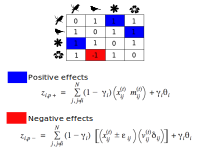
\includegraphics[width=\linewidth]{Sup_Figura_1.pdf}
  \vspace*{-7mm}
  \caption{Each effect between interacting species (\textit{+} or \textit{-}) in a community represented by an adjacency matrix of interactions are described by an adaptive peak. Each peak is influenced by the environmental factors of importance $\gamma_{i}$ favouring a trait value called $\theta{_i}$ and the ecological interactions which the positive effects favoured the species trait matching and the negative effect the trait decoupling due to the $\varepsilon_{ij}$. Finally, the sum of all the effects (positive and negatives) for a single species defines the final adaptive peak equations for that species}
  \label{supfig:1}
\end{figure}

\begin{figure}[H]
 \centering
  \includegraphics[width=\linewidth]{Sup_Figura_2.pdf}
  \vspace*{-7mm}
  \caption{Consistency test of expected frequency of exploitation interactions in a fully connected bipartite network with 50 species. For \textit{p} ranging from 0.01 to 1, we plot the expected and observed value of frequency of negative effects in the network. The expected frequency it's simply the value of \textit{p} used and the observed values are the frequency of interactions in the \textit{V} matrix. The value of \textit{p} used is a good proxy for the frequency of exploitation interactions in networks}
  \label{supfig:2}
\end{figure}

\begin{figure}[H]
 \centering
  \includegraphics[width=\linewidth]{Sup_Figura_3.pdf}
  \vspace*{-7mm}
  \caption{Four theoretical examples of coevolutionary dynamics showing \textit{Z}, the mean trait values of 10 species described by our main model in a theoretical fully connected bipartite adjacency matrix with different values of frequency of exploitation interactions \textit{f(Ch)} inserted in a mutualistic network. Each graph is a single simulation where we show the increase in trait disparity and the gradual formation of species traits aggregation as we insert a higher quantity of negative effects in a mutualistic network, drawing attention to the Y axis scale in \textit{the f(Ch) = 0.8} graph.}
  \label{supfig:3}
\end{figure}

\begin{figure}[H]
 \centering
  \includegraphics[width=\linewidth]{Sup_Figura_4.png}
  \vspace*{-7mm}
  \caption{Four theoretical examples of coevolutionary dynamics showing \textit{Z}, the mean trait values of 10 species described by our main model in a theoretical fully connected bipartite adjacency matrix with different values of frequency of exploitation interactions \textit{f(Ch)} inserted in a mutualistic network. Each graph is a single simulation where we show the increase in trait disparity and the gradual formation of species traits aggregation as we insert a higher quantity of negative effects in a mutualistic network, drawing attention to the Y axis scale in \textit{the f(Ch) = 0.8} graph.}
  \label{supfig:4}
\end{figure}

\begin{figure}[H]
 \centering
  \includegraphics[width = \linewidth, height = 17cm]{Sup_Figura_5.pdf}
  \vspace*{-7mm}
  \caption{Sensibility analysis showing our metrics with different equilibrium conditions to our simulations. Each point in the graph shows the Mean pairwise distance and clustering of species traits in three different trait equilibrium values: $10^{-4}, 10^{-6}$ e $10^{-8}$. We have 50 simulations for each scenario totaling 150 simulations.}
  \label{supfig:5}
\end{figure}

\begin{figure}[H]
 \centering
  \includegraphics[width = \linewidth, height = 17cm]{Sup_Figura_6.png}
  \vspace*{-7mm}
  \caption{Four theoretical examples of coevolutionary dynamics showing \textit{Z}, the mean trait values of 10 species described by our main model in a theoretical fully connected bipartite adjacency matrix with different values of frequency of exploitation interactions \textit{f(Ch)} inserted in a mutualistic network. Each graph is a single simulation where we show the increase in trait disparity and the gradual formation of species traits aggregation as we insert a higher quantity of negative effects in a mutualistic network, drawing attention to the Y axis scale in \textit{the f(Ch) = 0.8} graph.}
  \label{supfig:6}
\end{figure}
\end{singlespace}

\addcontentsline{toc}{subsection}{Code and data accessibility}
\subsection*{Code and data accessibility}
All the functions, scripts, results and figures used in the paper are available online in the GitHub platform in the \textit{coevo mut antag} repository. Additional to the code, you will find small guides and tutorials where we shown the basic process of simulation and how the main figures was generated. Also, we provide a link to the database's where all the empirical networks could be find and downloaded.

\begin{itemize}
    \item \href{https://github.com/lucascamacho/coevo_mut_antag}{GitHub repository}
    \item \href{http://www.web-of-life.es}{Web of Life website}
    \item \href{https://www.nceas.ucsb.edu/interactionweb/}{Interaction Web Data Base}
\end{itemize}

\addcontentsline{toc}{subsection}{References}
\begin{singlespace}
\subsection*{References}
\printbibliography[heading = none]

\end{singlespace}
\newpage

\end{document}